%% -----------------------------------------------------------------------
%% Modèle de thèse/mémoire/essai UQAC
%% 
%% Options de la classe:
%%   - times: pour utiliser Times/Helvetica plutôt que Computer Modern
%%   - these, memoire, essai, projetthese: crée une page titre libellée
%%        "thèse" (resp. "mémoire", "essai", etc.)
%%   - Toutes les options de la classe "book"
%% -----------------------------------------------------------------------
\documentclass[times,twoside,these]{uqac-these}

%% Pour utiliser les caractères accentués. Assurez-vous que
%% votre éditeur texte sauvegarde les fichiers en utilisant l'encodage UTF-8
\usepackage[utf8]{inputenc}

%% ------------------------
%% Quelques définitions
%% ------------------------

%% Titre du document. Ne pas l'écrire tout en majuscules!
\newcommand{\UqacTheseTitre}{Applications du convecteur temporel:
  une étude empirique}

%% Auteur du document
\newcommand{\UqacTheseAuteur}{Emmett Brown}

%% Date (mois année) du document
\newcommand{\UqacTheseDate}{Novembre 1955}

% Cette ligne évite une panoplie de warnings de pdflatex si on inclut
% des figures PDF récentes (version 1.6 et supérieures)
\pdfminorversion=7

% On ignore les warnings de pdflatex sur les "PDF page groups"
% (n'a aucun effet dans notre cas)
\pdfsuppresswarningpagegroup=1

%% ------------------------
%% Packages usuels
%% ------------------------

%% Pour les citations de type (Auteur, année) plutôt que [numéro].
%% Attention: la clé des références ne doit *pas* contenir le caractère ":"
%% (bug du package natbib)
\usepackage{natbib}

%% Pour interligne simple dans les listes (table des matières, etc.) et
%% double dans le reste
\usepackage{setspace}

%% Pour générer des PDF/A (le format demandé par l'UQAC lors du dépôt
%% final). Il est recommandé de décommenter cette ligne seulement pour
%% la production de l'ultime PDF du dépôt final.
%\usepackage[a-1b]{pdfx}

%% Pour ajouter des méta-données PDF et des hyperliens
\usepackage{hyperref}

%% Pour inclure des graphiques (via la commande \includegraphics)
\usepackage{graphicx}
\graphicspath{{fig/}}

%% Pour inclure des listings de code source
\usepackage{listings}
\lstset{
  language=Java,
  basicstyle=\ttfamily\small,
  columns=flexible,
  frame=single
}
\addto\captionsfrench{
  \renewcommand{\lstlistlistingname}{Liste des sources}
}
\addto\captionsenglish{
  \renewcommand{\lstlistlistingname}{List of Sources}
}

% Pour l'index
\makeindex

%% ------------------------
%% Création des méta-données PDF
%% ------------------------
\makeatletter
\newcommand{\UqacTheseVersion}{\@uqactheseversion}
\makeatother
\hypersetup{%
  pdfauthor = {\UqacTheseAuteur},
  pdftitle = {\UqacTheseTitre},
  pdfproducer = {Package uqac-these V\UqacTheseVersion}
}

\begin{document}
  
%% ------------------------
%% Création de la page titre
%% ------------------------
\title{\UqacTheseTitre}
\author{\UqacTheseAuteur}
\date{\UqacTheseDate}
\thispagestyle{empty}
\maketitle

%% ------------------------
%% Pages préliminaires
%% ------------------------
\frontmatter
\singlespacing
%% \chapter*{Avant-propos}

L'avant-propos doit être inscrit ici, à simple interligne, il est facultatif
et permet à l'auteur de faire état des raisons qui l'ont conduit à choisir
un sujet et du but qu'il vise ainsi que de l'ampleur et des limites de sa
recherche. Il peut également servir à remercier le directeur de recherche ou
toute autre personne. Mais, si tel est le cas, il faut intituler cette page
"REMERCIEMENTS" au lieu de "AVANT-PROPOS". L'avant-propos ne doit en aucun
cas remplacer l'introduction.

Velit amet diam pellentesque lectus ipsum,
lorem nibh congue est fringilla in id, aenean integer, tristique nunc ac
vehicula elementum, natoque rutrum venenatis. Turpis nisl venenatis. Mi
tincidunt placerat et semper et consectetuer, eu massa mi justo, velit
feugiat, sodales praesent ullamcorper ut eget nisl pretium. Bibendum quisque
massa posuere, convallis dolor id purus nulla, in velit ac, proin bibendum
nec magna wisi, et at est fugit. Dictum dui consectetuer elit venenatis
vestibulum, orci luctus justo ipsum, semper varius sed tortor magna mauris
non. Condimentum et vulputate amet vitae nunc, donec in dapibus, feugiat
mauris ipsum tellus, mauris integer wisi, nisl consequat phasellus. Montes
velit aliquet, viverra condimentum amet, ante consequat nulla ut mi quis,
lacus sed non ut nulla est nullam, neque nec ridiculus quam pellentesque id
tortor. Sit sem eu dolor duis ut
 %% Facultatif
\cleardoublepage
\addcontentsline{toc}{chapter}{\contentsname}
\tableofcontents
\cleardoublepage
\addcontentsline{toc}{chapter}{\listfigurename}
\listoffigures
\cleardoublepage
\addcontentsline{toc}{chapter}{\listtablename}
\listoftables
\cleardoublepage
\addcontentsline{toc}{chapter}{\lstlistlistingname}
\lstlistoflistings

%% ------------------------
%% Document principal
%% ------------------------
\mainmatter
\doublespacing
\chapter*{Résumé}

Lorem ipsum dolor sit amet, consectetur adipiscing elit. Aenean ac
ullamcorper mi. Vivamus non turpis odio. Cras vel mauris mauris. Vivamus
augue justo, fringilla vitae placerat a, rutrum placerat mi. Mauris in
ligula in velit aliquam sodales eu ac est. Phasellus elementum interdum
lectus id congue. Nullam eget rutrum augue.

Quisque ut tellus nulla. Phasellus ut turpis quis erat semper pharetra.
Donec consectetur vehicula dui id pretium. In et massa lectus. Nulla mattis
pulvinar convallis. Etiam at odio velit. Phasellus eleifend, neque vel
euismod rutrum, turpis orci gravida velit, vel placerat arcu lectus quis
nisl. Vivamus vel mauris justo. Donec facilisis facilisis sem, in vestibulum
quam imperdiet eget.

%% L'introduction n'est pas numérotée mais elle apparaît dans la table
%% des matières
\chapter*{Introduction}

Lorem ipsum dolor sit amet, consectetur adipiscing elit. Aenean ac
ullamcorper mi. Vivamus non turpis odio. Cras vel mauris mauris. Vivamus
augue justo, fringilla vitae placerat a, rutrum placerat mi. Mauris in
ligula in velit aliquam sodales eu ac est. Phasellus elementum interdum
lectus id congue. Nullam eget rutrum augue.

Quisque ut tellus nulla. Phasellus ut turpis quis erat semper pharetra.
Donec consectetur vehicula dui id pretium. In et massa lectus. Nulla mattis
pulvinar convallis. Etiam at odio velit. Phasellus eleifend, neque vel
euismod rutrum, turpis orci gravida velit, vel placerat arcu lectus quis
nisl. Vivamus vel mauris justo. Donec facilisis facilisis sem, in vestibulum
quam imperdiet eget. Sed tortor justo, adipiscing a tincidunt at, pharetra
vitae felis. Ut quis orci leo, id suscipit leo. Maecenas tincidunt lectus et
risus tempus non tristique libero tempor. In arcu sapien, suscipit ac tempor
eu, venenatis ut tellus. Nullam metus felis, tempor id scelerisque tempor,
fermentum non nisl. Nulla viverra ultricies neque sit amet facilisis.

Lorem ipsum dolor sit amet, consectetur adipiscing elit. Aenean ac
ullamcorper mi. Vivamus non turpis odio. Cras vel mauris mauris. Vivamus
augue justo, fringilla vitae placerat a, rutrum placerat mi. Mauris in
ligula in velit aliquam sodales eu ac est. Phasellus elementum interdum
lectus id congue. Nullam eget rutrum augue.

Quisque ut tellus nulla. Phasellus ut turpis quis erat semper pharetra.
Donec consectetur vehicula dui id pretium. In et massa lectus. Nulla mattis
pulvinar convallis. Etiam at odio velit. Phasellus eleifend, neque vel
euismod rutrum, turpis orci gravida velit, vel placerat arcu lectus quis
nisl. Vivamus vel mauris justo. Donec facilisis facilisis sem, in vestibulum
quam imperdiet eget. Sed tortor justo, adipiscing a tincidunt at, pharetra
vitae felis. Ut quis orci leo, id suscipit leo. Maecenas tincidunt lectus et
risus tempus non tristique libero tempor. In arcu sapien, suscipit ac tempor
eu, venenatis ut tellus. Nullam metus felis, tempor id scelerisque tempor,
fermentum non nisl. Nulla viverra ultricies neque sit amet facilisis.
  

\chapter{Titre d'un chapitre}

Lorem ipsum dolor sit amet, consectetur adipiscing elit. Nulla pellentesque
ante ut velit tincidunt rhoncus. Ut aliquam consectetur tempor. Nulla luctus
nisl at urna placerat tristique. Suspendisse tempus iaculis nisl at
suscipit. Class aptent taciti sociosqu ad litora torquent per conubia
nostra, per inceptos himenaeos. Nulla vel libero placerat enim scelerisque
interdum quis nec tortor. Quisque fermentum rhoncus dolor sodales
sollicitudin. Donec quis mi nisi, quis blandit nulla. Pellentesque varius
ipsum ut tortor pretium vel eleifend diam iaculis. Aenean nulla ligula,
congue in placerat non, varius ut nibh.

Exemples de citations: blabla la théorie des types
\citep{DBLPjournals/jsyml/Turing48,DBLPjournals/ai/Lenat82}. Si on mentionne
le nom, ne pas le répéter dans la citation: comme le disait
\citet{DBLPjournals/jsyml/Turing48}, ou même
\citet{DBLPconf/afips/SolomonP76}.

\section{Une première section}

Praesent diam libero, tincidunt vel interdum at, luctus id nisl. Ut egestas
nisi a elit ullamcorper tempus. Sed nisl enim, fermentum et consequat ac,
aliquam quis diam. Nulla elementum, purus nec fermentum vestibulum, justo
ligula tempus orci, non dignissim ligula orci id nulla. Integer placerat
posuere quam sit amet congue. Proin eleifend, turpis mollis gravida
tristique, justo nisl semper nunc, quis pellentesque neque ligula eu quam.
Cras a felis urna. Suspendisse dui sem, ullamcorper sed viverra a, varius id
odio. Nullam in nisi id massa tempor varius cursus id neque. Curabitur
ultrices fermentum purus tempor scelerisque. Maecenas in iaculis tellus.
Nulla et sollicitudin quam. Pellentesque sed mi at massa facilisis auctor.
Quisque non metus massa.

\subsection{Un sous-titre}

Fusce et dui at mi semper aliquam in sed ipsum. Etiam in urna enim.
Vestibulum arcu tellus, venenatis ac sollicitudin vel, sagittis eget nisl.
Mauris ut nunc ipsum. Phasellus ut magna a nisi aliquam scelerisque ut a
sapien. Ut lectus leo, faucibus vitae sagittis ac, sagittis posuere tortor.
Nulla id odio dui, eu pharetra massa. Etiam bibendum posuere elit, sit amet
tristique leo blandit sed. Voyez par exemple la figure \ref{fig:formes}.

\begin{figure}
  \begin{center}
  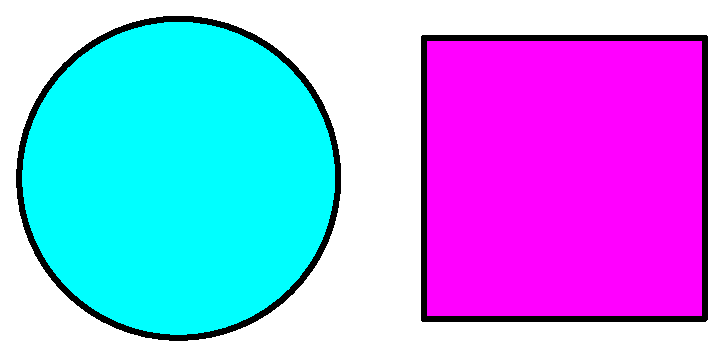
\includegraphics[width=3in]{carre-et-cercle}
  \end{center}
  \caption{Des formes géométriques}
  \label{fig:formes}
\end{figure}

Pellentesque molestie laoreet gravida. Curabitur egestas mollis libero, in
posuere turpis malesuada at. Donec egestas nunc sed justo eleifend
tincidunt. Vestibulum dignissim lobortis nisl, quis gravida tortor pulvinar
id. In ac nisi metus, in varius felis. Morbi semper aliquam turpis sed
vehicula. Nam neque libero, condimentum sed gravida ut, egestas ut nibh.
Lorem ipsum dolor sit amet, consectetur adipiscing elit.

\subsection{Un autre sous-titre}

Sed lacus mi, aliquet et elementum id, tincidunt in leo. Donec id ligula
erat, sit amet condimentum justo. Aliquam mi risus, molestie quis egestas
id, consequat nec erat. Aenean hendrerit augue quis massa consequat eu
ultricies lorem tincidunt. Lorem ipsum dolor sit amet, consectetur
adipiscing elit. Donec ornare ligula quis nunc tincidunt euismod. Phasellus
eget mi elit. Suspendisse neque est, placerat ac tincidunt ut, dapibus non
ante. Morbi varius, orci sed interdum euismod, risus purus dapibus magna,
non convallis augue augue eget elit. Comme le dit le tableau
\ref{tab:villes}. Duis ut feugiat massa. Duis at nunc non lacus rhoncus
porta vitae vel felis. Etiam eu euismod libero. Vestibulum ante ipsum primis
in faucibus orci luctus et ultrices posuere cubilia Curae; Fusce facilisis
dui eu augue ultrices non venenatis lectus viverra.

\begin{table}
  \caption{Un tableau avec un titre}
  \begin{center}
    \begin{tabular}{|c|c|c|}
      \hline
      Ville & Année & Naissance \\
      \hline\hline
      Chicoutimi & 2000 & 1936 \\
      \hline
      Jonquière & 2001 & 1944 \\
      \hline
      La Baie & 2002 & 1952 \\
      \hline
  \end{tabular}
  \label{tab:villes}
  \end{center}
\end{table}

\section{Une seconde section}

Curabitur quis arcu urna, sed laoreet magna. Proin ut sollicitudin arcu.
Suspendisse rhoncus, mauris sit amet lacinia interdum, justo erat auctor
nisi, at eleifend orci neque id ipsum. Aliquam rutrum accumsan dolor, sit
amet elementum mauris gravida vel. In hac habitasse platea dictumst. Mauris
sit amet diam velit, non rhoncus lorem. Suspendisse pulvinar, dolor a tempor
cursus, nibh nisl tincidunt augue, non aliquet mauris enim vitae massa.
Vestibulum ante ipsum primis in faucibus orci luctus et ultrices posuere
cubilia Curae; Suspendisse potenti. Nullam rutrum, dolor quis molestie
sollicitudin, ipsum orci condimentum nibh, nec tincidunt sem nisi eget leo.
Ut porta metus neque, id tincidunt est. Phasellus mollis porta euismod.

\[
  \sum_{i=0}^n i = \frac{n(n+1)}{2}
\]

Morbi pellentesque, urna in gravida porta, neque nisl imperdiet lorem, at
molestie lacus dolor aliquam eros. Duis vel interdum ante. Aenean dignissim,
dolor sed accumsan vulputate, elit ipsum mollis mauris, ultricies cursus
lorem enim sit amet elit. Suspendisse congue dolor vel urna semper at mattis
leo cursus. Phasellus cursus, odio ut gravida auctor, nisi lacus iaculis
erat, in interdum elit dolor et est. Nunc eleifend ullamcorper erat, lacinia
suscipit augue luctus vel. Etiam quis nisl vel turpis sodales bibendum vitae
ac velit. Pellentesque accumsan lacus massa. Nunc sollicitudin massa
adipiscing neque placerat vestibulum.

\subsection{Un sous-titre}

Quisque a lorem sit amet diam sollicitudin lobortis vitae ac massa. Mauris
id eros sed enim egestas eleifend at vel nunc. Vivamus risus erat, pretium
quis convallis sit amet, pellentesque id sem. Cras massa metus, luctus eu
molestie adipiscing, condimentum sit amet mauris. Sed euismod consectetur
blandit. Nunc et nunc sed nunc tempor aliquam. Class aptent taciti sociosqu
ad litora torquent per conubia nostra, per inceptos himenaeos. Vestibulum
rhoncus feugiat orci, non venenatis mauris lobortis quis. Aenean
sollicitudin tempor diam, at feugiat leo adipiscing ut. Vivamus fermentum
semper diam vitae ultrices. Nulla consequat ullamcorper nulla ac consequat.

\subsection{Un dernier sous-titre}

Duis sed augue et sem tempus tempor. Fusce ut bibendum diam. In orci tellus,
porttitor ut euismod porttitor, lacinia in lacus. Aenean augue sem, porta
eget ultricies id, ornare a purus. Nulla facilisi. Donec non dignissim
purus. Nam arcu velit, placerat ut convallis at, laoreet nec sem. Phasellus
ac nisl et tellus adipiscing varius. Phasellus consequat tristique est, at
mattis magna ullamcorper at. Donec bibendum, arcu ac scelerisque vulputate,
massa erat porta sapien, a iaculis erat ligula aliquam ligula. Nam eget elit
lacus. Donec vel arcu ut dolor consequat pretium. Suspendisse gravida
vestibulum arcu, sit amet viverra sem feugiat consequat. Aliquam ultrices
gravida condimentum. Sed turpis magna, blandit in porttitor quis, interdum
eu erat.

Etiam tincidunt arcu sed nulla adipiscing vel tempus erat luctus. Nulla
convallis hendrerit feugiat. Curabitur et vehicula ante. Mauris mattis enim
et lorem consectetur venenatis sollicitudin sapien pharetra. Nulla dictum
mattis tincidunt. Nullam urna ipsum, aliquet consequat semper eu, vestibulum
at dolor. Morbi libero tellus, dignissim ut elementum a, rutrum nec lacus.
Pellentesque id venenatis turpis. Pellentesque habitant morbi tristique
senectus et netus et malesuada fames ac turpis egestas. Nunc rutrum mollis
sodales. Cum sociis natoque penatibus et magnis dis parturient montes,
nascetur ridiculus mus. Fusce urna ante, facilisis sit amet posuere vitae,
interdum quis felis. Quisque sollicitudin, urna et vestibulum feugiat, elit
lectus egestas tellus, a ultrices nulla tellus mattis mi. Vivamus id tellus
ac quam aliquet vestibulum vehicula non dui.

\chapter{Titre d'un autre chapitre}

Lorem ipsum dolor sit amet, consectetur adipiscing elit. Nulla pellentesque
ante ut velit tincidunt rhoncus. Ut aliquam consectetur tempor. Nulla luctus
nisl at urna placerat tristique. Suspendisse tempus iaculis nisl at
suscipit. Class aptent taciti sociosqu ad litora torquent per conubia
nostra, per inceptos himenaeos. Nulla vel libero placerat enim scelerisque
interdum quis nec tortor. Quisque fermentum rhoncus dolor sodales
sollicitudin. Donec quis mi nisi, quis blandit nulla. Pellentesque varius
ipsum ut tortor pretium vel eleifend diam iaculis. Aenean nulla ligula,
congue in placerat non, varius ut nibh.

Exemples de citations: blabla la théorie des types
\citep{DBLPjournals/jsyml/Turing48}. Si on mentionne le nom, ne pas le
répéter dans la citation: comme le disait
\citet{DBLPjournals/jsyml/Turing48}.

\section{Une première section}

Praesent diam libero, tincidunt vel interdum at, luctus id nisl. Ut egestas
nisi a elit ullamcorper tempus. Sed nisl enim, fermentum et consequat ac,
aliquam quis diam. Nulla elementum, purus nec fermentum vestibulum, justo
ligula tempus orci, non dignissim ligula orci id nulla. Integer placerat
posuere quam sit amet congue. Proin eleifend, turpis mollis gravida
tristique, justo nisl semper nunc, quis pellentesque neque ligula eu quam.
Cras a felis urna. Suspendisse dui sem, ullamcorper sed viverra a, varius id
odio. Nullam in nisi id massa tempor varius cursus id neque. Curabitur
ultrices fermentum purus tempor scelerisque. Maecenas in iaculis tellus.
Nulla et sollicitudin quam. Pellentesque sed mi at massa facilisis auctor.
Quisque non metus massa.

\subsection{Un sous-titre}

Fusce et dui at mi semper aliquam in sed ipsum. Etiam in urna enim.
Vestibulum arcu tellus, venenatis ac sollicitudin vel, sagittis eget nisl.
Mauris ut nunc ipsum. Phasellus ut magna a nisi aliquam scelerisque ut a
sapien. Ut lectus leo, faucibus vitae sagittis ac, sagittis posuere tortor.
Nulla id odio dui, eu pharetra massa. Etiam bibendum posuere elit, sit amet
tristique leo blandit sed.

Pellentesque molestie laoreet gravida. Curabitur egestas mollis libero, in
posuere turpis malesuada at. Donec egestas nunc sed justo eleifend
tincidunt. Vestibulum dignissim lobortis nisl, quis gravida tortor pulvinar
id. In ac nisi metus, in varius felis. Morbi semper aliquam turpis sed
vehicula. Nam neque libero, condimentum sed gravida ut, egestas ut nibh.
Lorem ipsum dolor sit amet, consectetur adipiscing elit.

\subsection{Un autre sous-titre}

Sed lacus mi, aliquet et elementum id, tincidunt in leo. Donec id ligula
erat, sit amet condimentum justo. Aliquam mi risus, molestie quis egestas
id, consequat nec erat. Aenean hendrerit augue quis massa consequat eu
ultricies lorem tincidunt. Lorem ipsum dolor sit amet, consectetur
adipiscing elit. Donec ornare ligula quis nunc tincidunt euismod. Phasellus
eget mi elit. Suspendisse neque est, placerat ac tincidunt ut, dapibus non
ante. Morbi varius, orci sed interdum euismod, risus purus dapibus magna,
non convallis augue augue eget elit. Duis ut feugiat massa. Duis at nunc non
lacus rhoncus porta vitae vel felis. Etiam eu euismod libero. Vestibulum
ante ipsum primis in faucibus orci luctus et ultrices posuere cubilia Curae;
Fusce facilisis dui eu augue ultrices non venenatis lectus viverra.

\section{Une seconde section}

Curabitur quis arcu urna, sed laoreet magna. Proin ut sollicitudin arcu.
Suspendisse rhoncus, mauris sit amet lacinia interdum, justo erat auctor
nisi, at eleifend orci neque id ipsum. Aliquam rutrum accumsan dolor, sit
amet elementum mauris gravida vel. In hac habitasse platea dictumst. Mauris
sit amet diam velit, non rhoncus lorem. Suspendisse pulvinar, dolor a tempor
cursus, nibh nisl tincidunt augue, non aliquet mauris enim vitae massa.
Vestibulum ante ipsum primis in faucibus orci luctus et ultrices posuere
cubilia Curae; Suspendisse potenti. Nullam rutrum, dolor quis molestie
sollicitudin, ipsum orci condimentum nibh, nec tincidunt sem nisi eget leo.
Ut porta metus neque, id tincidunt est. Phasellus mollis porta euismod.

\[
  \sum_{i=0}^n i = \frac{n(n+1)}{2}
\]

Morbi pellentesque, urna in gravida porta, neque nisl imperdiet lorem, at
molestie lacus dolor aliquam eros. Duis vel interdum ante. Aenean dignissim,
dolor sed accumsan vulputate, elit ipsum mollis mauris, ultricies cursus
lorem enim sit amet elit. Suspendisse congue dolor vel urna semper at mattis
leo cursus. Phasellus cursus, odio ut gravida auctor, nisi lacus iaculis
erat, in interdum elit dolor et est. Nunc eleifend ullamcorper erat, lacinia
suscipit augue luctus vel. Etiam quis nisl vel turpis sodales bibendum vitae
ac velit. Pellentesque accumsan lacus massa. Nunc sollicitudin massa
adipiscing neque placerat vestibulum.

\subsection{Un sous-titre}

Quisque a lorem sit amet diam sollicitudin lobortis vitae ac massa. Mauris
id eros sed enim egestas eleifend at vel nunc. Vivamus risus erat, pretium
quis convallis sit amet, pellentesque id sem. Cras massa metus, luctus eu
molestie adipiscing, condimentum sit amet mauris. Sed euismod consectetur
blandit. Nunc et nunc sed nunc tempor aliquam. Class aptent taciti sociosqu
ad litora torquent per conubia nostra, per inceptos himenaeos. Vestibulum
rhoncus feugiat orci, non venenatis mauris lobortis quis. Aenean
sollicitudin tempor diam, at feugiat leo adipiscing ut. Vivamus fermentum
semper diam vitae ultrices. Nulla consequat ullamcorper nulla ac consequat.

\subsection{Un dernier sous-titre}

Duis sed augue et sem tempus tempor. Fusce ut bibendum diam. In orci tellus,
porttitor ut euismod porttitor, lacinia in lacus. Aenean augue sem, porta
eget ultricies id, ornare a purus. Nulla facilisi. Donec non dignissim
purus. Nam arcu velit, placerat ut convallis at, laoreet nec sem. Phasellus
ac nisl et tellus adipiscing varius. Phasellus consequat tristique est, at
mattis magna ullamcorper at. Donec bibendum, arcu ac scelerisque vulputate,
massa erat porta sapien, a iaculis erat ligula aliquam ligula. Nam eget elit
lacus. Donec vel arcu ut dolor consequat pretium. Suspendisse gravida
vestibulum arcu, sit amet viverra sem feugiat consequat. Aliquam ultrices
gravida condimentum. Sed turpis magna, blandit in porttitor quis, interdum
eu erat.

Etiam tincidunt arcu sed nulla adipiscing vel tempus erat luctus. Nulla
convallis hendrerit feugiat. Curabitur et vehicula ante. Mauris mattis enim
et lorem consectetur venenatis sollicitudin sapien pharetra. Nulla dictum
mattis tincidunt. Nullam urna ipsum, aliquet consequat semper eu, vestibulum
at dolor. Morbi libero tellus, dignissim ut elementum a, rutrum nec lacus.
Pellentesque id venenatis turpis. Pellentesque habitant morbi tristique
senectus et netus et malesuada fames ac turpis egestas. Nunc rutrum mollis
sodales. Cum sociis natoque penatibus et magnis dis parturient montes,
nascetur ridiculus mus. Fusce urna ante, facilisis sit amet posuere vitae,
interdum quis felis. Quisque sollicitudin, urna et vestibulum feugiat, elit
lectus egestas tellus, a ultrices nulla tellus mattis mi. Vivamus id tellus
ac quam aliquet vestibulum vehicula non dui.

%% ...
%% Ajoutez autant de commandes include qu'il y a de chapitres à
%% inclure dans votre document
%% ...
%% La conclusion n'est pas numérotée
\chapter*{Conclusion}

Lorem ipsum dolor sit amet, consectetur adipiscing elit. Aenean ac
ullamcorper mi. Vivamus non turpis odio. Cras vel mauris mauris. Vivamus
augue justo, fringilla vitae placerat a, rutrum placerat mi. Mauris in
ligula in velit aliquam sodales eu ac est. Phasellus elementum interdum
lectus id congue. Nullam eget rutrum augue.

Quisque ut tellus nulla. Phasellus ut turpis quis erat semper pharetra.
Donec consectetur vehicula dui id pretium. In et massa lectus. Nulla mattis
pulvinar convallis. Etiam at odio velit. Phasellus eleifend, neque vel
euismod rutrum, turpis orci gravida velit, vel placerat arcu lectus quis
nisl. Vivamus vel mauris justo. Donec facilisis facilisis sem, in vestibulum
quam imperdiet eget. Sed tortor justo, adipiscing a tincidunt at, pharetra
vitae felis. Ut quis orci leo, id suscipit leo. Maecenas tincidunt lectus et
risus tempus non tristique libero tempor. In arcu sapien, suscipit ac tempor
eu, venenatis ut tellus. Nullam metus felis, tempor id scelerisque tempor,
fermentum non nisl. Nulla viverra ultricies neque sit amet facilisis.
  


%% ------------------------
%% Pages liminaires
%% ------------------------
\backmatter
%% Style des références bibliographiques
\bibliographystyle{theseuqam}

%% Liste des fichiers source pour la bibliograhpie.
%% On peut inclure plus d'un fichier en séparant leurs noms par des
%% virgules.
\bibliography{bibliographie}

%% Décommenter cette ligne pour afficher l'index
% \printindex
\end{document}
